\documentclass{beamer}
\usetheme{metropolis}
\usepackage{graphicx}
\usepackage{mathtools}
\usepackage{subfig}
\usepackage{tcolorbox}
\title{Algebra-Based Physics: Electricity, Magnetism, and Modern Physics (PHYS135B): Unit 3}
\author{Jordan Hanson}
\institute{Whittier College Department of Physics and Astronomy}

\begin{document}
\maketitle

\section{Summary}

\begin{frame}{Unit 3 Summary}
\begin{enumerate}
\item \textbf{Magnetostatics I: Chapters 22.1 - 22.4}
\begin{enumerate}
\item Magnets, ferromagnetic and electromagnetic
\item Magnetic fields and field lines, force on moving charge
\item Magnetic application: \alert{mass spectrometry}
\end{enumerate}
\item \textbf{Magnetostatics II: Chapters 22.7 - 22.9}
\begin{enumerate}
\item Forces and torques on conductors with current
\item Amp\`{e}re's Law: magnetic fields are created by currents
\item Magnetic application: \alert{fusion reactors}
\end{enumerate}
\end{enumerate}
\end{frame}

\section{Magnets and magnetic fields}

\begin{frame}{Magnets and magnetic fields}
\footnotesize
\begin{tcolorbox}[colback=white,colframe=gray,title=Review of the Origin of Electric and Magnetic Fields]
On the origin of magnetic fields and forces they exert on charge:\\ \\
\url{https://www.youtube.com/watch?v=s94suB5uLWw} \\ \\
On the origin of electric fields and forces they exert on charge:\\ \\
\url{https://youtu.be/mdulzEfQXDE?si=euGvVjKPT33_E-fI}
\end{tcolorbox}
\small
\textbf{Key points:}
\begin{itemize}
\item Some elements are magnetic or can be magnetized
\item Current creates magnetic fields
\item Current exerts force on moving charge and current
\end{itemize}
\end{frame}

\begin{frame}{Magnets and magnetic fields}
What is a cross-product and how does it work? \\ \vspace{0.25cm}
\begin{figure}
\centering
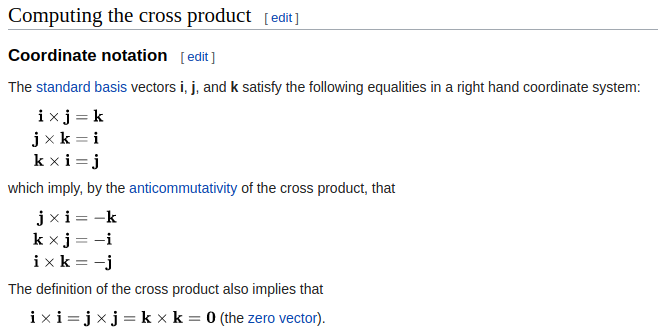
\includegraphics[width=0.75\textwidth]{figures/crossP.png}
\caption{\label{fig:crossP} The cross-product is a way of multiplying unit vectors.}
\end{figure}
\textbf{Professor:} several examples on board.
\end{frame}

\begin{frame}{Magnets and magnetic fields}
Let $\vec{v} = 2\hat{i}$ and $w = -2 \hat{j}$.  What is $\vec{v} \times \vec{w}$?
\begin{itemize}
\item A: $-4 \hat{k}$
\item B: $4 \hat{k}$
\item C: $-2 \hat{i}$
\item D: $2 \hat{j}$
\end{itemize}
\end{frame}

\begin{frame}{Magnets and magnetic fields}
Let $\vec{v} = 3\hat{j}$ and $w = 5 \hat{k}$.  What is $\vec{v} \times \vec{w}$?
\begin{itemize}
\item A: $15 \hat{i}$
\item B: $5 \hat{j}$
\item C: $3 \hat{i}$
\item D: $15 \hat{k}$
\end{itemize}
\end{frame}

\begin{frame}{Magnets and magnetic fields}
Let $\vec{v} = 3\hat{i} \times 3\hat{j}$ and $w = 2 \hat{k}$.  What is $\vec{v} \times \vec{w}$?
\begin{itemize}
\item A: $-6 \hat{j} + 6\hat{k}$
\item B: $-6 \hat{j} + 6\hat{i}$
\item C: $6 \hat{j} + 6\hat{i}$
\item D: $6 \hat{k} + 6\hat{i}$
\end{itemize}
\end{frame}

\begin{frame}{Magnets and magnetic fields}
\textbf{Group exercise:} Compute the following cross product:
\begin{align}
\vec{v} &= 2\hat{i}-2\hat{j} \\
\vec{w} &= 4\hat{j}-4\hat{i} \\
\vec{v} \times \vec{w} &= ??
\end{align}
\end{frame}

\begin{frame}{Magnets and magnetic fields}
\small
\begin{tcolorbox}[colback=white,colframe=black!100!black,title=The Lorentz Force]
\alert{Let a particle with charge $q$ and velocity $\vec{v}$ move through a \textit{magnetic field} $\vec{B}$.  The \textbf{Lorentz force} on the charged particle is
\begin{equation}
\vec{F} = q\vec{v} \times \vec{B}
\label{eq:Lorentz}
\end{equation}
If $\theta$ is the angle between $\vec{v}$ and $\vec{B}$, the magnitude of $\vec{F}$ is
\begin{equation}
F = qvB \sin\theta
\end{equation}}
\footnotesize
\end{tcolorbox}
\textit{As a helpful memory tool, we have the right-hand rule to remember the direction of the cross-product.}  \textbf{The units of the magnetic field are the Telsa}, after Nikola Tesla.  We also have the Gauss which is $10^{-4}$ Tesla.
\end{frame}

\begin{frame}{Magnets and magnetic fields}
\begin{figure}
\centering
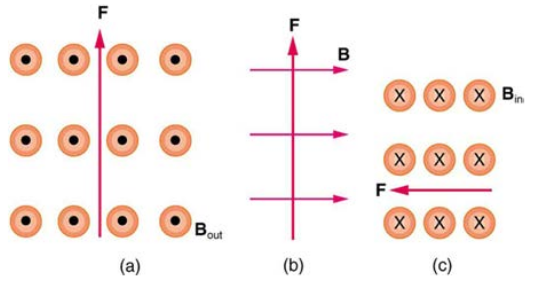
\includegraphics[width=0.75\textwidth]{figures/lorentzProblem.png}
\caption{\label{fig:lorentzProblem} Three different magnetic field and charge scenarios.  The vector $\vec{F}$ is the direction of the Lorentz force, and the magnetic field is uniform.  A dot indicates that the magnetic field is coming out of the page, and an x indicates that the field is going into the page.}
\end{figure}
\end{frame}

\begin{frame}{Magnets and magnetic fields}
\begin{columns}[T]
\begin{column}{0.3\textwidth}
In which of the diagrams is a positively charged particle moving to the left?
\begin{itemize}
\item A: A
\item B: B
\item C: C
\item D: Double WAT
\end{itemize}
\end{column}
\begin{column}{0.7\textwidth}
\begin{figure}
\centering
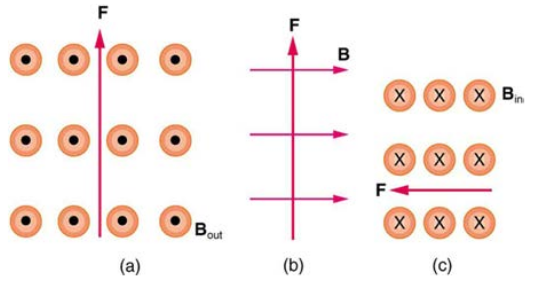
\includegraphics[width=0.75\textwidth]{figures/lorentzProblem.png}
\caption{\label{fig:lorentzProblem2} Three different magnetic field and charge scenarios.}
\end{figure}
\end{column}
\end{columns}
\end{frame}

\begin{frame}{Magnets and magnetic fields}
\begin{columns}[T]
\begin{column}{0.3\textwidth}
In which of the diagrams is a positively charged particle moving upwards?
\begin{itemize}
\item A: A
\item B: B
\item C: C
\item D: Double WAT
\end{itemize}
\end{column}
\begin{column}{0.7\textwidth}
\begin{figure}
\centering
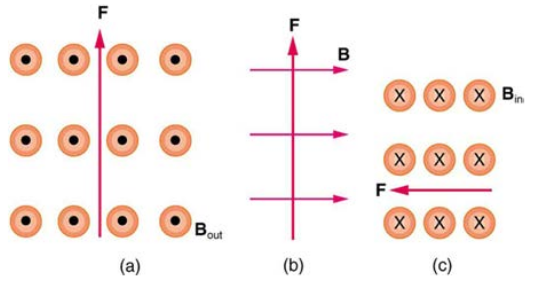
\includegraphics[width=0.75\textwidth]{figures/lorentzProblem.png}
\caption{\label{fig:lorentzProblem3} Three different magnetic field and charge scenarios.}
\end{figure}
\end{column}
\end{columns}
\end{frame}

\begin{frame}{Magnets and magnetic fields}
\begin{columns}[T]
\begin{column}{0.3\textwidth}
In which of the diagrams is a negatively charged particle moving into the page?
\begin{itemize}
\item A: A
\item B: B
\item C: C
\item D: Double WAT
\end{itemize}
\end{column}
\begin{column}{0.7\textwidth}
\begin{figure}
\centering
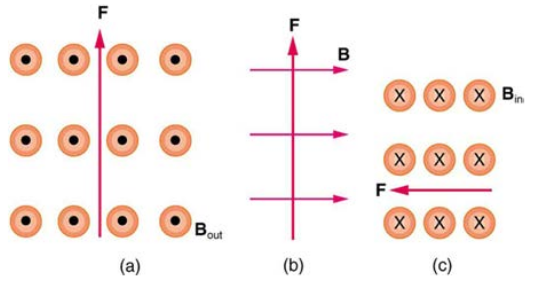
\includegraphics[width=0.75\textwidth]{figures/lorentzProblem.png}
\caption{\label{fig:lorentzProblem4} Three different magnetic field and charge scenarios.}
\end{figure}
\end{column}
\end{columns}
\end{frame}

\begin{frame}{Magnets and magnetic fields}
\begin{columns}[T]
\begin{column}{0.3\textwidth}
In which of the diagrams is a negatively charged particle moving to the right?
\begin{itemize}
\item A: A
\item B: B
\item C: C
\item D: Double WAT
\end{itemize}
\end{column}
\begin{column}{0.7\textwidth}
\begin{figure}
\centering
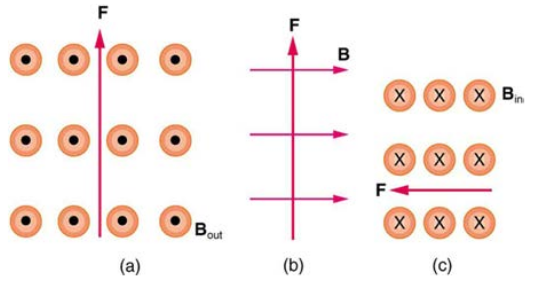
\includegraphics[width=0.75\textwidth]{figures/lorentzProblem.png}
\caption{\label{fig:lorentzProblem5} Three different magnetic field and charge scenarios.}
\end{figure}
\end{column}
\end{columns}
\end{frame}

\begin{frame}{Magnets and magnetic fields}
A theorem for the magnitude of the cross-product:  Let $\vec{a}$ and $\vec{b}$ be vectors and $\theta$ be the angle between them.  The magnitude of the cross-product is
\begin{equation}
|\vec{a} \times \vec{b}| =  a b \sin\theta
\end{equation}
Thus, the magnitude of the Lorentz force is
\begin{equation}
F_{\rm L} = q v B \sin\theta
\end{equation}
The angle $\theta$ is between the velocity and the magnetic field.
\end{frame}

\begin{frame}{Magnets and magnetic fields}
Suppose a positively charged particle $q$ moves with an initial velocity $\vec{v} = v \hat{i}$, and there is a uniform magnetic field $\vec{B} = -B\hat{k}$.  At this moment, what is the direction of the force on $q$?
\begin{itemize}
\item A: $\hat{i}$
\item B: $\hat{j}$
\item C: $\hat{k}$
\item D: $-\hat{k}$
\end{itemize}
\end{frame}

\begin{frame}{Magnets and magnetic fields}
The force on the positively charged particle $q$ in the $\hat{k}$-direction eventually causes the velocity to be $\vec{v} = v\hat{j}$.  The uniform magnetic field is still $\vec{B} = -B\hat{k}$.  At this moment, what is the direction of the force on $q$?
\begin{itemize}
\item A: $\hat{i}$
\item B: $\hat{j}$
\item C: $\hat{k}$
\item D: $-\hat{i}$
\end{itemize}
\end{frame}

\begin{frame}{Magnets and magnetic fields}
\small
\textbf{\alert{The charge experiences uniform circular motion.}} At each moment, the acceleration is \textit{perpendicular} to the direction.
\begin{figure}
\centering
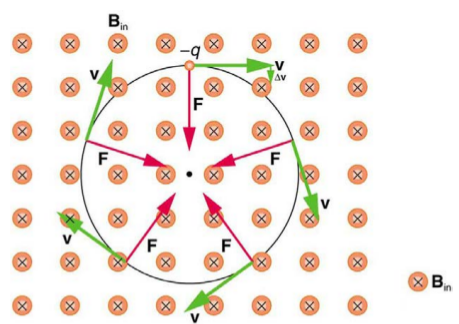
\includegraphics[width=0.4\textwidth]{figures/qmcircle.png}
\caption{\label{fig:qm} The situation is depicted here with $-q$ (changes direction).}
\end{figure}
\textbf{Recall} centripetal acceleration, in two equations:
\begin{equation}
F_{\rm C} = \frac{m v^2}{r} = m r \omega^2
\end{equation}
\end{frame}

\begin{frame}{Magnets and magnetic fields}
\small
\textbf{Recall} centripetal acceleration, in two equations:
\begin{equation}
F_{\rm C} = \frac{m v^2}{r} = m r \omega^2
\end{equation}
Assume the Lorentz force remains perpendicular to velocity, and set the centripetal force equal to Lorentz force magnetiude:
\begin{align}
\frac{mv^2}{r} &= qv B \\
qB &= \frac{mv}{r} \\
r &= \frac{mv}{qB}
\end{align}
Thus, the radius of curvature is connected to ratio of mass, charge, velocity, and field strength.  \textit{What is a scientific application of this?}
\end{frame}

\section{Magnetic Applications I: Mass Spectrometry}

\begin{frame}{Magnetic Applications I: Mass Spectrometry}
\footnotesize
\textbf{\alert{Mass spectrometry.}} A simplified picture of mass spectrometry involves measuring the radius of curvature of ions in a B-field.
\begin{figure}
\centering
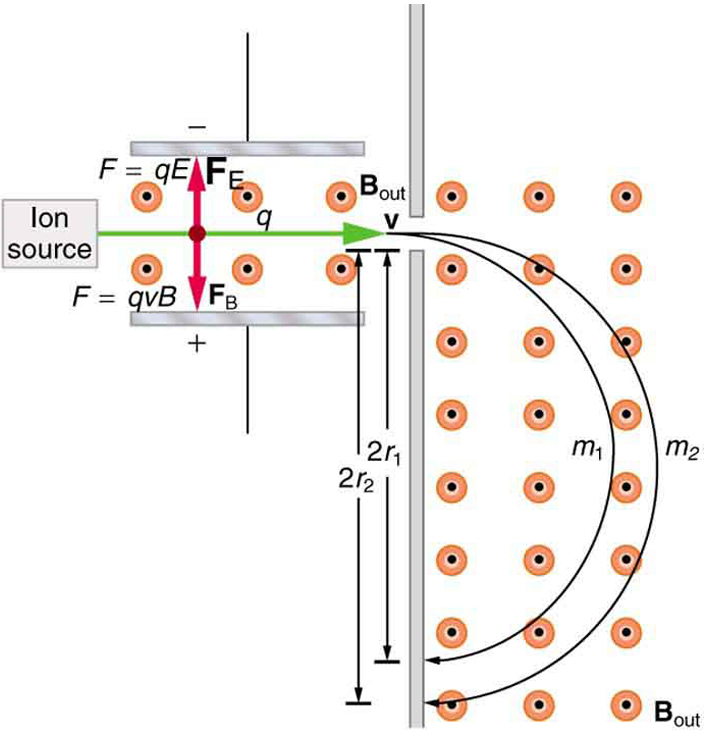
\includegraphics[width=0.35\textwidth]{figures/mass_spec.jpeg}
\caption{\label{fig:mass} \footnotesize (a) Within the ion source, molecules are turned into an ionized gas, and accelerated through a capacitor.  (b) The capacitor creates a uniform E-field, and a coil of current surrounds the capacitor to create a uniform B-field.  The E and B-fields are perpendicular. (c) Ions leave the \textit{velocity selector} into an area with just the B-field.}
\end{figure}
\end{frame}

\begin{frame}{Magnetic Applications I: Mass Spectrometry}
\begin{columns}[T]
\begin{column}{0.5\textwidth}
\begin{figure}
\centering
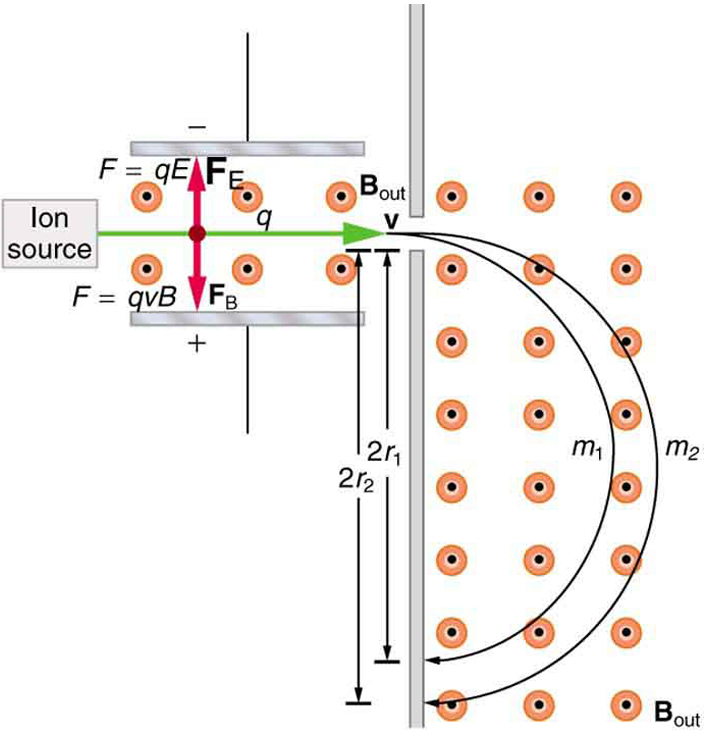
\includegraphics[width=0.9\textwidth]{figures/mass_spec.jpeg}
\caption{\label{fig:mass2} A simplified picture of a mass spectrometer.}
\end{figure}
\end{column}
\begin{column}{0.5\textwidth}
\small
\begin{enumerate}
\item Show that if $v = E/B$, the velocity in the \textit{velocity selector} is constant.
\item If $E = 100$ V/m, and $B = 50$ gauss (5 mT), what velocity is required from the ion source?
\item If $q$ is the equivalent of two electrons (2\textit{e}), and $m$ is 100 amu\footnote{1 amu = $1.66 \times 10^{-27}$ kg, and 1\textit{e} = $1.67 \times 10^{-19}$ C.}, what is the radius observed after the velocity selector?
\end{enumerate}
\end{column}
\end{columns}
\end{frame}

\begin{frame}{Magnetic Applications I: Mass Spectrometry}
Within $\approx 1$ \%, what result did you obtain?
\begin{itemize}
\item A: 0.02 m
\item B: 0.2 m
\item C: 2.0 m
\item D: 20 m
\end{itemize}
\end{frame}

\begin{frame}{Magnetic Applications I: Mass Spectrometry}
If all other variables remained the same, what would the radius of curvature be if $m$ decreased to 50 amu?
\begin{itemize}
\item A: 10 m
\item B: 1.0 m
\item C: 0.1 m
\item D: 0.01 m
\end{itemize}
\footnotesize
(It is not necessary to repeat the calculation.  Treat this as a scaling problem.)
\end{frame}

\begin{frame}{Magnetic Applications I: Mass Spectrometry}
\footnotesize
\textbf{Notes on the Lorentz force:}
\begin{enumerate}
\item Magnetic fields do no work.
\begin{itemize}
\item Work is defined as
\begin{equation}
W = \vec{F} \cdot \vec{x}
\end{equation}
\item Insert the Lorentz force for $\vec{F}$:
\begin{equation}
W = q\vec{v} \times \vec{B} \cdot \vec{x}
\end{equation}
\item $\vec{v} \times \vec{B}$ is perpendicular to $\vec{x}$, which is parallel to $\vec{v}$.
\item $W = 0$, because the dot-product of perpendicular vectors is zero.
\end{itemize}
\item The radio of E to B-fields is a \textit{velocity}, $v = E/B$?  What happens for a moving observer?  We will postpone this discussion until we cover \textit{inductors.}
\end{enumerate}
\end{frame}

\begin{frame}{Magnets and magnetic fields}
\begin{figure}
\centering
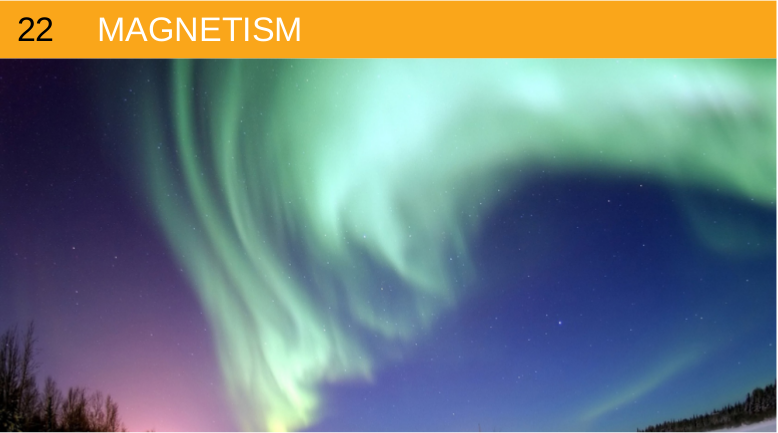
\includegraphics[width=0.9\textwidth]{figures/aurora.png}
\caption{\label{fig:aurora} The aurora borealis, or northern lights.}
\end{figure}
\end{frame}

\begin{frame}{Magnets and magnetic fields}
\textbf{\alert{A cool talk on the aurora borealis}} (\textit{time permitting}):
\url{https://youtu.be/czMh3BnHFHQ} \\
\begin{figure}
\centering
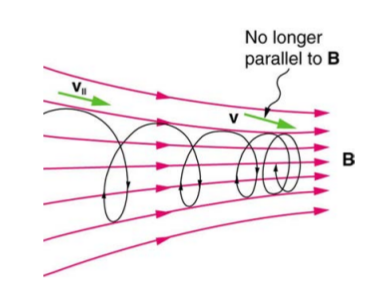
\includegraphics[width=0.35\textwidth]{figures/mag1.png}
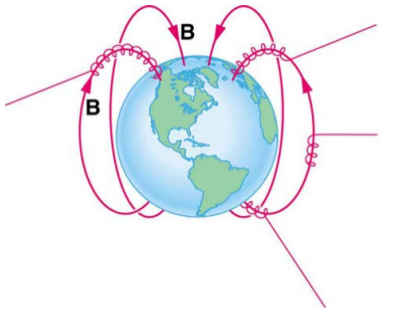
\includegraphics[width=0.35\textwidth]{figures/mag2.png}
\end{figure}
One un-explained piece: what does it mean for the electrons and protons to \textit{high-five} the neutral oxygen and nitrogen atoms?
\end{frame}

\section{Force and Torque on a Current Carrying Conductor}

\begin{frame}{Force and Torque on a Current Carrying Conductor}
Introduction to magnetic forces on current-carrying conductors: \\ \vspace{0.5cm}
\url{https://youtu.be/5fqwJyt4Lus} \\
\begin{figure}
\centering
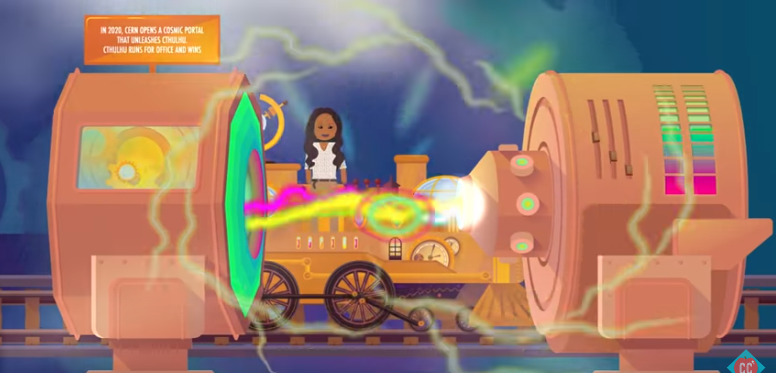
\includegraphics[width=0.7\textwidth]{figures/pbs.png}
\end{figure}
\end{frame}

\begin{frame}{Force and Torque on a Current Carrying Conductor}
\textbf{\alert{The Lorentz force}} also effects currents in conductors.
\begin{figure}
\centering
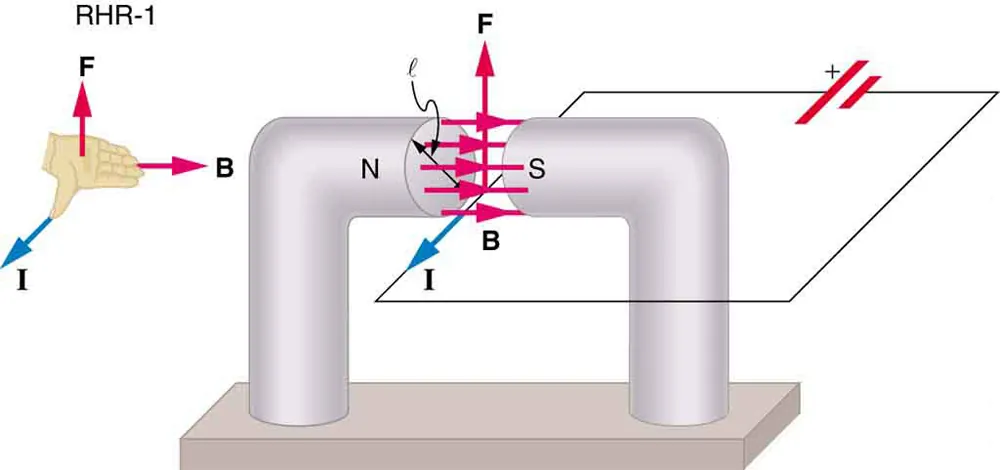
\includegraphics[width=0.65\textwidth]{figures/lorentz_wire.png}
\caption{\label{fig:lorentz_wire} \footnotesize A B-field exerts a force on a wire carrying current.}
\end{figure}
\scriptsize
\begin{columns}[T]
\begin{column}{0.5\textwidth}
\begin{align}
F_q &= q v_{\rm d} B \sin\theta \\
F_{\rm tot} &= N q v_{\rm d} B \sin\theta \\
N &= nV \\
N & = n A L
\end{align}
\end{column}
\begin{column}{0.5\textwidth}
\begin{align}
F_{\rm tot} &= \left(n q A v_{\rm d}\right) L B \sin\theta \\
F_{\rm tot} &= I L B \sin\theta \\
F_{\rm tot} &= I \vec{L} \times \vec{B}
\end{align}
\end{column}
\end{columns}
\end{frame}

\begin{frame}{Force and Torque on a Current Carrying Conductor}
\begin{columns}[T]
\begin{column}{0.5\textwidth}
\footnotesize
\textbf{\alert{What is number density?}} Number density converts a volume to the number of objects in the volume:
\begin{equation}
\boxed{N = nV}
\end{equation}
Suppose the Milky Way galaxy is a disc of diameter 100,000 light-years and height of 1,000 light years.  We think there are about $10^{11}$ stars in the Milky Way.  What is the number density of stars in the galaxy?
\begin{itemize}
\item A: $10$ stars per light year
\item B: $1$ star per light year
\item C: $0.1$ stars per light year
\item D: $0.01$ stars per light year
\end{itemize}
\end{column}
\begin{column}{0.5\textwidth}
\begin{figure}
\centering
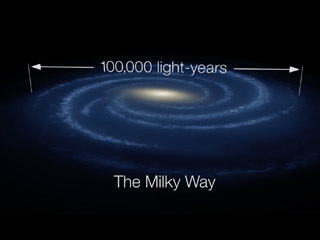
\includegraphics[width=0.9\textwidth]{figures/milky_way.jpg}
\caption{\label{fig:milky} An artist's conception of the diameter of the Milky Way.}
\end{figure}
\end{column}
\end{columns}
\end{frame}

\begin{frame}{Force and Torque on a Current Carrying Conductor}
\begin{columns}[T]
\begin{column}{0.4\textwidth}
\footnotesize
\textbf{\alert{Why does $nqAv_{\rm d}$ equal current?}} Consider the geometry of charges flowing through a conductor:
\begin{align}
I &= \frac{\Delta Q}{\Delta t} \\
\Delta Q &= N q = n V q \\
\Delta Q &= n A L q \\
L &= v_{\rm d} \Delta t \\
I &= \frac{n A L q v_{\rm d}}{L} \\
\Aboxed{I &= n A L q v_{\rm d}}
\end{align}
The $n$ must be the number density of \textit{free charges.}
\end{column}
\begin{column}{0.6\textwidth}
\begin{figure}
\centering
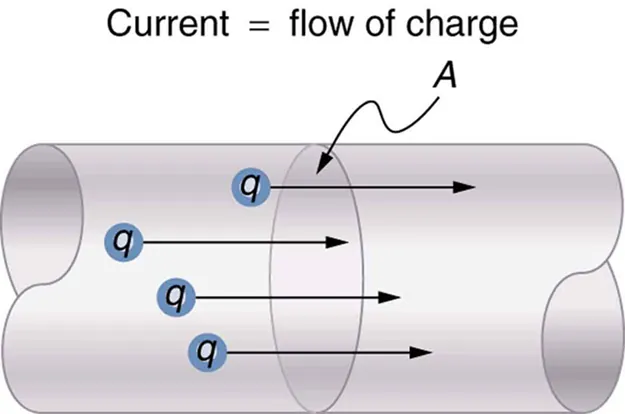
\includegraphics[width=0.55\textwidth]{figures/current_1.png}
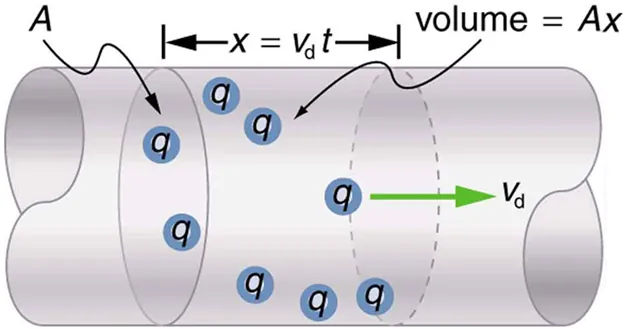
\includegraphics[width=0.55\textwidth]{figures/current_0.png}
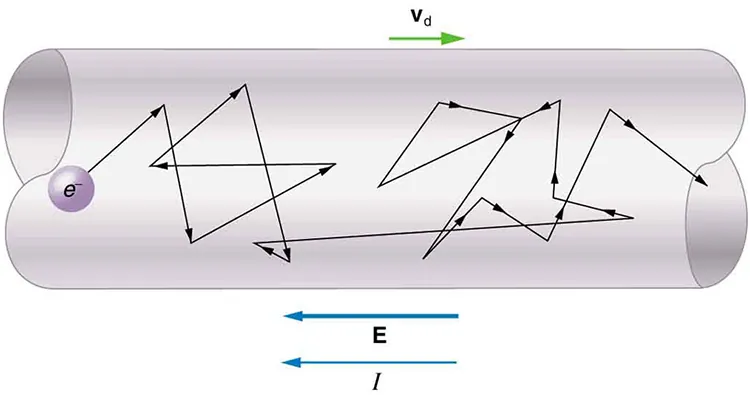
\includegraphics[width=0.55\textwidth]{figures/current_2.png}
\caption{\label{fig:current} Simple picture of current.}
\end{figure}
\end{column}
\end{columns}
\end{frame}

\begin{frame}{Force and Torque on a Current Carrying Conductor}
\small
\begin{tcolorbox}[colback=white,colframe=gray,title=Lorentz Force on Current Carrying Conductor]
\alert{The force on a current $I$ of vector length $\vec{L}$ within a magnetic field $\vec{B}$ is
\begin{equation}
\vec{F} = I \vec{L} \times \vec{B}
\end{equation}
If $\theta$ is the angle between $\vec{L}$ and $\vec{B}$, the magnitude of $\vec{F}$ is 
\begin{equation}
F = ILB \sin\theta
\end{equation}}
\end{tcolorbox}
\footnotesize
\textit{When using this concept, remember:}
\begin{itemize}
\item The units of Tesla are N m$^{-1}$ A$^{-1}$
\item The vector $\vec{L}$ has the length of the conductor
\item The vector $\vec{L}$ has the direction of positive current
\end{itemize}
\end{frame}

\begin{frame}{Force and Torque on a Current Carrying Conductor}
A 1 m wire carries a 0.5 A current in the x-direction.  A B-field of 0.01 T is in the y-direction.  What is the magnitude of the force on the wire?
\begin{itemize}
\item A: $5 \times 10^{-2}$ N
\item B: $5 \times 10^{-3}$ N
\item C: $5 \times 10^{-1}$ N
\item D: $5 \times 10^{-4}$ N
\end{itemize}
\end{frame}

\begin{frame}{Force and Torque on a Current Carrying Conductor}
A 1 m wire carries a 0.5 A current in the x-direction ($\hat{i}$).  A B-field of 0.01 T is in the y-direction ($\hat{j}$).  In what direction is the force?
\begin{itemize}
\item A: $\hat{k}$
\item B: $-\hat{k}$
\item C: $-\hat{j}$
\item D: $\hat{j}$
\end{itemize}
\end{frame}

\begin{frame}{Force and Torque on a Current Carrying Conductor}
A loop of wire is in the x-y plane, centered at the origin.  It carries a current in the counter-clockwise direction.  A uniform B-field in the \textbf{\alert{z-direction}} surrounds the wire.  The loop of current will
\begin{itemize}
\item A: Rotate
\item B: Move to the left
\item C: Move to the right
\item D: Remain stationary
\end{itemize}
\end{frame}

\begin{frame}{Force and Torque on a Current Carrying Conductor}
A loop of wire is in the x-y plane, centered at the origin.  It carries a current in the counter-clockwise direction.  A uniform B-field in the \textbf{\alert{y-direction}} surrounds the wire.  The loop of current will
\begin{itemize}
\item A: Rotate
\item B: Move to the left
\item C: Move to the right
\item D: Remain stationary
\end{itemize}
\end{frame}

\begin{frame}{Force and Torque on a Current Carrying Conductor}
\begin{columns}[T]
\begin{column}{0.4\textwidth}
\footnotesize
A magnetohydrodynamic (MHD) pump system is shown in Fig. \ref{fig:MHD}.  A current is passed through a liquid, and the liquid passes through a B-field.  Since the angle $\theta$ between $\vec{L}$ and $\vec{B}$ is 90 degrees, $\boxed{F = ILB}$.  What B-field is required to produce a pumping force of $10^{-3}$ N, if the diameter of the pipe is 1 cm, and the achievable current is 0.1 A?
\end{column}
\begin{column}{0.6\textwidth}
\begin{figure}
\centering
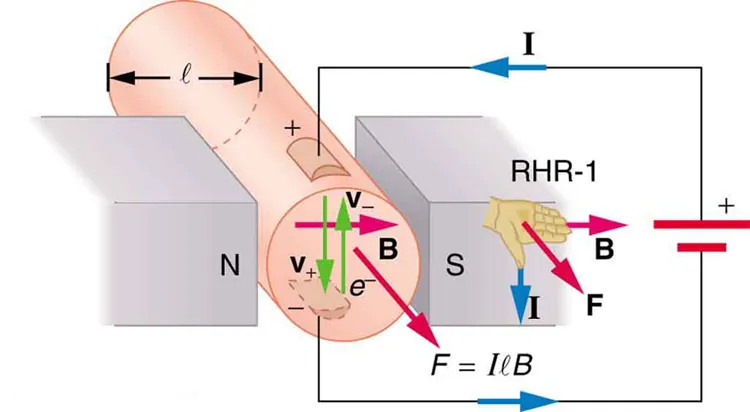
\includegraphics[width=0.85\textwidth]{figures/MHD.png}
\caption{\label{fig:MHD} \footnotesize Simple picture of an MHD pump.}
\end{figure}
\normalsize
\begin{itemize}
\item A: $0.01$ T
\item B: $0.1$ T
\item C: $1.0$ T
\item D: $10.0$ T
\end{itemize}
\end{column}
\end{columns}
\end{frame}

\begin{frame}{Force and Torque on a Current Carrying Conductor}
\small
Returning to the \textbf{rotating loop of current}, notice it implies a \textit{torque:}
\begin{figure}
\centering
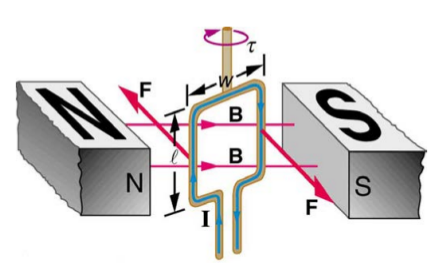
\includegraphics[width=0.5\textwidth]{figures/loop.png}
\caption{\label{fig:loop} In a loop of current in a uniform magnetic field, we find forces going the opposite directions.}
\end{figure}
\textbf{\alert{Torque}} can be defined like:
\begin{equation}
\boxed{\vec{\tau} = \vec{r} \times \vec{F}}
\end{equation}
\end{frame}

\begin{frame}{Force and Torque on a Current Carrying Conductor}
\small
Returning to the \textbf{rotating loop of current}, notice it implies a \textit{torque:}
\begin{figure}
\centering
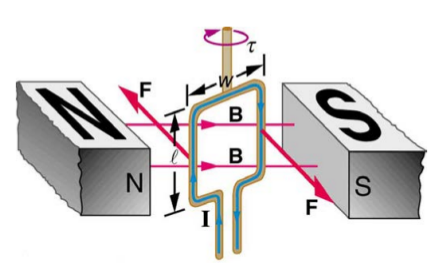
\includegraphics[width=0.5\textwidth]{figures/loop.png}
\caption{\label{fig:loop2} A loop of current in a B-field.}
\end{figure}
The magnitude follows the usual pattern for cross-products.  In Fig. \ref{fig:loop2}, $r = w/2$, and $\theta$ is the angle between $F$ and $r$.
\begin{equation}
\tau = rF\sin\theta
\end{equation}
\end{frame}

\begin{frame}{Force and Torque on a Current Carrying Conductor}
\begin{figure}
\centering
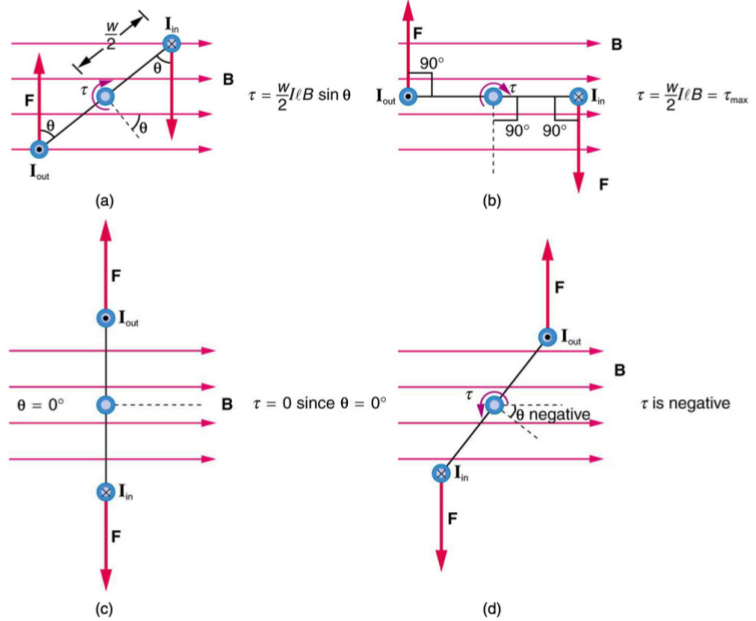
\includegraphics[width=0.7\textwidth]{figures/torque.png}
\caption{\label{fig:loop3} (a) Torque is positive (in). (b) Torque is maximally positve. (c) Torque is zero. (d) Torque is negative.}
\end{figure}
\end{frame}

\begin{frame}{Force and Torque on a Current Carrying Conductor}
\small
The \textbf{loop of current}, experiences a \textit{torque} that is proportional to loop area, number of turns (coils), current, B-field magnitude, and the sine of the angle between the loop and the force.
\begin{align}
\vec{\tau} &= \vec{r} \times \vec{F} \\
\tau_{\rm L,R} &= r F \sin\theta \\
\tau &= \tau_{\rm L} + \tau_{\rm R} \\
\tau &= \frac{w}{2}F\sin\theta + \frac{w}{2}\sin\theta = wF\sin\theta \\
F &= I w B \\
\tau &= I w^2 B = I A B \sin\theta \\
\tau &= N I A B \sin\theta
\end{align}
\end{frame}

\begin{frame}{Force and Torque on a Current Carrying Conductor}
Recall that $\boxed{\tau = N I A B \sin\theta}$.  What is the maximum torque experienced by a coil of $N = 200$ turns of wire carrying 2.0 A with area $A = 0.2$ m$^2$ in a 2.0 T B-field?
\begin{itemize}
\item A: 0 N m
\item B: 16 N m
\item C: 160 N
\item D: 160 N m
\end{itemize}
\footnotesize
What is the \textit{minimum torque}?
\end{frame}

\begin{frame}{Force and Torque on a Current Carrying Conductor}
How do we avoid the problem of \textit{negative torque}?  If $\tau$ is negative when $\theta$ is between 180 and 359 degrees, one idea is to periodically disconnect the circuit with \textit{brushes.}
\begin{figure}
\centering
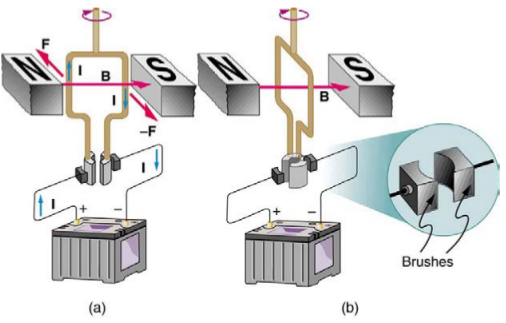
\includegraphics[width=0.6\textwidth]{figures/motor.png}
\caption{\label{fig:motor} Torque can be used to drive a motor.}
\end{figure}
\end{frame}

\begin{frame}{Force and Torque on a Current Carrying Conductor}
Recall that $\tau = N I A B \sin\theta$.  Suppose that $\tau = 0$ when $180 < \theta < 359$ (degrees), because $I = 0$. Suppose further that when $\theta = 90$ (degrees), the torque is 160 N m.  What is the torque when $\theta = 30$ (degrees)?
\begin{itemize}
\item A: 160 N m
\item B: 80 N m
\item C: 160/$\sqrt{2}$ N m
\item D: 80 N
\end{itemize}
\hrulefill \\
\footnotesize
An example of DIY physics experiment to illustrate this concept:
\url{https://youtu.be/WI0pGk0MMhg?si=D-YjbydOmKPzPJlG}
\end{frame}

\section{Amp\`{e}re's Law: Magnetic Fields Created by Current}

\begin{frame}{Amp\`{e}re's Law: Magnetic Fields Created by Current}
\textbf{\alert{One version of Amp\`{e}re's Law}} relates the \textit{magnetic field} created by a \textit{current} in a long straight wire:
\begin{tcolorbox}[colback=white,colframe=gray,title=Amp\`{e}re's Law]
\alert{Let the permeability of free space be $\mu_0 = 4\pi \times 10^{-7}$ T m A$^{-1}$. The magnetic field $\vec{B}$ a distance $r$ from a long, straight wire carrying a current $I$ is given by
\begin{equation}
\vec{B} = \frac{\mu_0 I}{2\pi r} \hat{\phi}
\end{equation}}
\end{tcolorbox}
\footnotesize
How do we sort out the direction, $\hat{\phi}$?
\end{frame}

\begin{frame}{Amp\`{e}re's Law: Magnetic Fields Created by Current}
\textbf{\alert{One version of Amp\`{e}re's Law}} relates the \textit{magnetic field} created by a \textit{current} in a long straight wire:
\begin{figure}
\centering
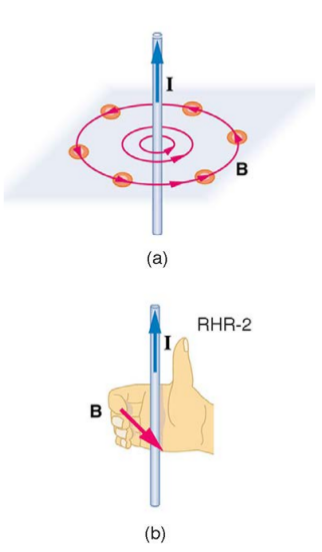
\includegraphics[width=0.35\textwidth,trim=0cm 10cm 0cm 0cm,clip=true]{figures/rhr2.png}
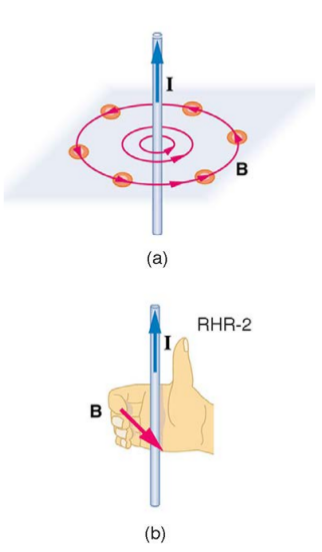
\includegraphics[width=0.35\textwidth,trim=0cm 0cm 0cm 10cm,clip=true]{figures/rhr2.png}
\caption{\label{fig:amp} (a) The B-field encircles the current ($\hat{\phi}$). (b) Put thumb in direction of current, curled fingers reveal B-field direction.}
\end{figure}
\end{frame}

\begin{frame}{Amp\`{e}re's Law: Magnetic Fields Created by Current}
Two wires are 1 cm apart, and the length of each is 100 cm.  Each carries a current of 1 A in the same direction.  What is the B-field of the left wire at the right wire?  What is the B-field of the right wire at the left wire?  Assume the currents are in the plane of the page and moving upwards.
\begin{itemize}
\item A: 2 Gauss out of the page, 2 Gauss out of the page
\item B: 1 Gauss into the page, 1 Gauss out of the page
\item C: 2 Gauss into the page, 2 Gauss out of the page
\item D: 2 Gauss out of the page, 2 Gauss into the page
\end{itemize}
\end{frame}

\begin{frame}{Amp\`{e}re's Law: Magnetic Fields Created by Current}
Two wires are 1 cm apart, and the length of each is 100 cm.  Each carries a current of 1 A in the same direction.  What is the force of the left wire on the right wire?  What is the force of the right wire on the left wire?  Assume the currents are in the plane of the page and moving upwards.
\begin{itemize}
\item A: $2\times 10^{-4}$ N (left), $2\times 10^{-4}$ N (right)
\item B: $2\times 10^{-4}$ N (right), $2\times 10^{-4}$ N (right)
\item C: $2\times 10^{-4}$ N (left), $2\times 10^{-4}$ N (left)
\item D: $1\times 10^{-4}$ N (left), $1\times 10^{-4}$ N (right)
\end{itemize}
\end{frame}

\begin{frame}{Amp\`{e}re's Law: Magnetic Fields Created by Current}
\begin{figure}
\centering
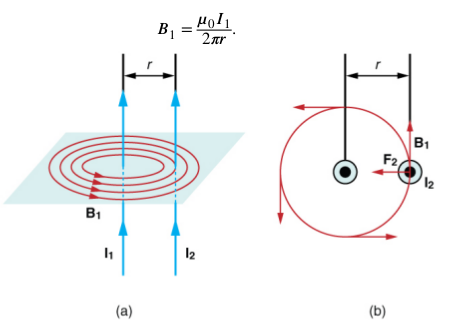
\includegraphics[width=0.45\textwidth]{figures/amp.png}
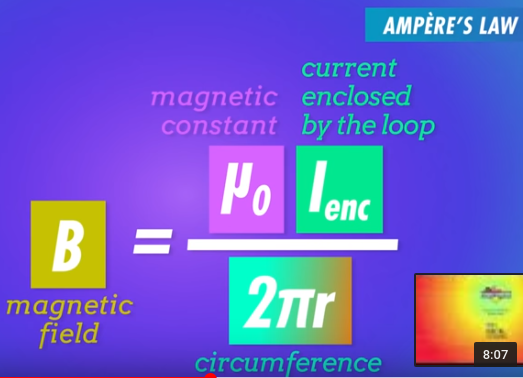
\includegraphics[width=0.45\textwidth]{figures/amplaw.png}
\caption{\label{fig:amp2} (a) The force of the left wire on the right wire attracts the right wire to the left wire.  (b)  Amp\`{e}re's Law summarized in our PBS Crash Course content.}
\end{figure}
\footnotesize
\textbf{One awesome final project idea:} DIY demonstration of Amp\`{e}re's Law.
\end{frame}

\begin{frame}{Amp\`{e}re's Law: Magnetic Fields Created by Current}
\begin{figure}
\centering
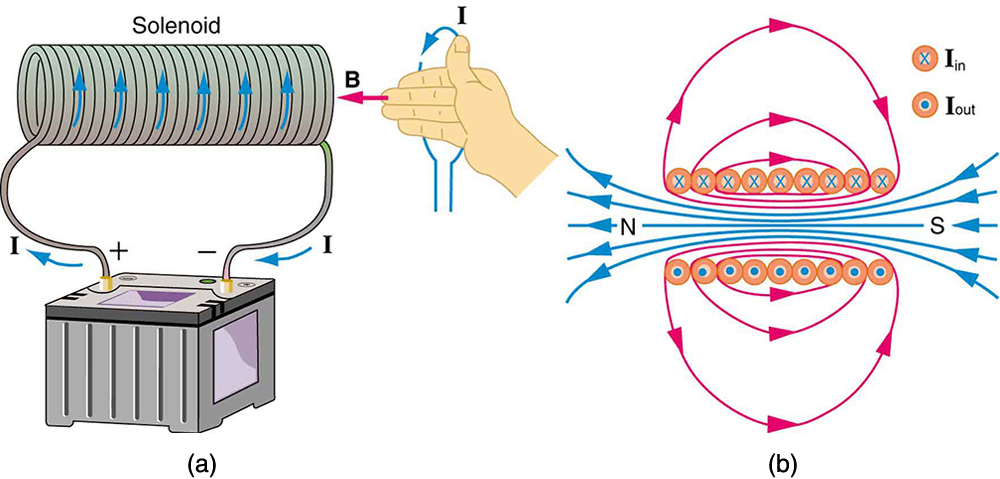
\includegraphics[width=0.85\textwidth]{figures/solenoid.jpeg}
\caption{\label{fig:solenoid1} A solenoid is an application of Amp\`{e}re's Law.}
\end{figure}
\end{frame}

\begin{frame}{Amp\`{e}re's Law: Magnetic Fields Created by Current}
\textbf{\alert{Amp\`{e}re's Law}} may be used to calculate the B-field in Fig. \ref{fig:solenoid1}.
\begin{tcolorbox}[colback=white,colframe=gray,title=Magnetic Field of a Solenoid]
\alert{Let the permeability of free space be $\mu_0 = 4\pi \times 10^{-7}$ T m A$^{-1}$.  Let $N$ parallel loops of wire with current $I$ be arranged concentrically along a distance $\vec{L} = L\hat{k}$, and let $n = N/L$.  This arrangement is called a \textit{solenoid}, and the magnetic field $\vec{B}$ everywhere inside it is
\begin{equation}
\vec{B} = \mu_0 n I \hat{k} \label{eq:solenoid}
\end{equation}}
\end{tcolorbox}
\end{frame}

\section{PhET Activity: Solenoids}

\begin{frame}{PhET Activity: Solenoids}
PhET simulation illustrating solenoids (\alert{run the CheerpJ browser compatible version}): \\ \vspace{0.5cm}
\small
\url{https://phet.colorado.edu/en/simulations/generator}
\begin{itemize}
\item Click the Electromagnet tab along the top line.
\item Click Show Field Meter in the grey box on the right side.
\item Use the DC battery as the current source, and assume a constant resistance (current is proportional to voltage).  Place the Field Meter inside the solenoid, and leave the number of loops constant.
\item Create a graph of B-field strength versus voltage, in steps of 1V, from $-10$ V to $10$ V.  Is the result linear?  How is this explained by Amp\`{e}re's Law and Eq. \ref{eq:solenoid}?
\end{itemize}
\end{frame}

\begin{frame}{PhET Activity: Solenoids}
PhET simulation illustrating solenoids (\alert{run the CheerpJ browser compatible version}): \\ \vspace{0.5cm}
\small
\url{https://phet.colorado.edu/en/simulations/generator}
\begin{itemize}
\item Click the Generator tab along the top line.
\item Activate the water spigot at left to spin the magnetic field.
\item Is the fact that the bulb lights up explained by Amp\`{e}re's Law?  In what ways is this experimental setup qualitatively different or similar to the Electromagnet experiment?
\end{itemize}
\textbf{We will now perform a laboratory activity based on the simulations.}
\end{frame}


\section{Magnetic Applications II: Nuclear Fusion}

\begin{frame}{Magnetic Applications II: Nuclear Fusion}
\textbf{\alert{Tokamaks}} provide magnetic containment of charged plasma.
\begin{figure}
\centering
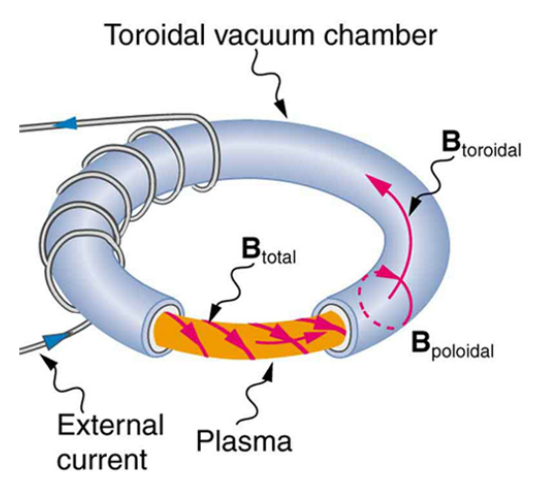
\includegraphics[width=0.6\textwidth]{figures/tokamak.png}
\caption{\label{fig:tokamak} The tokamak contains high-energy plasma.}
\end{figure}
\end{frame}

\begin{frame}{Magnetic Applications II: Nuclear Fusion}
\small
\begin{columns}[T]
\begin{column}{0.5\textwidth}
\begin{enumerate}
\item First, the external current creates a \textit{toroidal} magnetic field.
\item Use the right hand rule for positive current to show that the toroidal field should be counter-clockwise
\item Suppose a positively charged particle is injected into the toroidal field with velocity $\vec{v}$.  Suppose at least one component of the velocity is tangent to the counter-clockwise direction.\end{enumerate}
\end{column}
\begin{column}{0.5\textwidth}
\begin{figure}
\centering
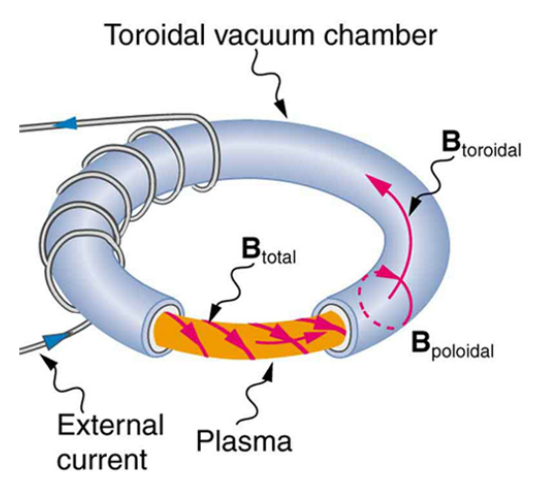
\includegraphics[width=0.9\textwidth]{figures/tokamak.png}
\caption{\label{fig:tokamak2} The tokamak contains high-energy plasma.}
\end{figure}
\end{column}
\end{columns}
\end{frame}

\begin{frame}{Magnetic Applications II: Nuclear Fusion}
\small
\begin{columns}[T]
\begin{column}{0.5\textwidth}
\begin{enumerate}
\item How will the positively charged particle begin to move?
\item Use the right hand rule for currents to predict the direction of the \textit{poloidal} B-field created by the ions.
\item Note how the \textit{poloidal} and \textit{toroidal} fields add together to form the spiral field.
\item  Can a positvely charged particle to escape?  Think about the Lorentz force and the cross product of $\vec{v} \times \vec{B}$.
\end{enumerate}
\end{column}
\begin{column}{0.5\textwidth}
\begin{figure}
\centering
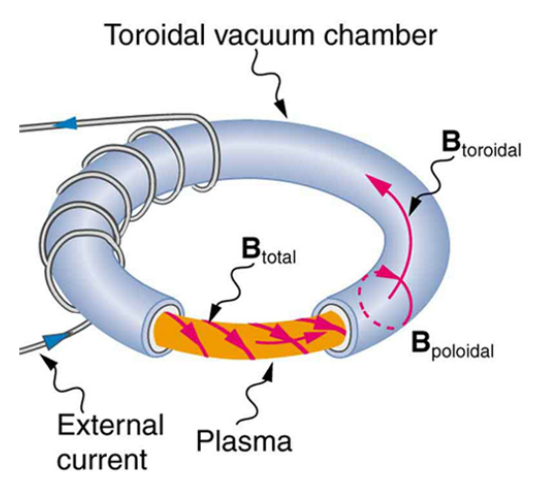
\includegraphics[width=0.9\textwidth]{figures/tokamak.png}
\caption{\label{fig:tokamak3} The tokamak contains high-energy plasma.}
\end{figure}
\end{column}
\end{columns}
\end{frame}

\section{Conclusion}

\begin{frame}{Unit 3 Summary}
\begin{enumerate}
\item \textbf{Magnetostatics I: Chapters 22.1 - 22.4}
\begin{enumerate}
\item Magnets, ferromagnetic and electromagnetic
\item Magnetic fields and field lines, force on moving charge
\item Magnetic application: \alert{mass spectrometry}
\end{enumerate}
\item \textbf{Magnetostatics II: Chapters 22.7 - 22.9}
\begin{enumerate}
\item Forces and torques on conductors with current
\item Amp\`{e}re's Law: magnetic fields are created by currents
\item Magnetic application: \alert{fusion reactors}
\end{enumerate}
\end{enumerate}
\end{frame}

\end{document}
